%particles
\newcommand{\jpsi}{\rm J/$\psi$}
\newcommand{\psip}{$\psi^\prime$}
\newcommand{\jpsiDY}{\rm J/$\psi$\,/\,DY}
\newcommand{\chic}{$\chi_{\rm c}$}
\newcommand{\pip}{$\pi^{+}$}
\newcommand{\pim}{$\pi^{-}$}
\newcommand{\pizero}{$\pi^{0}$}
\newcommand{\kap}{K$^{+}$}
\newcommand{\kam}{K$^{-}$}
\newcommand{\pbar}{$\rm\overline{p}$}
\newcommand{\ccbar}{\ensuremath{\mathrm{c\overline{c}}}}
\newcommand{\bbbar}{\ensuremath{\mathrm{b\overline{b}}}}
\newcommand{\Dzero}{\ensuremath{\mathrm{D^{0}}}}
\newcommand{\Dzerobar}{\ensuremath{\mathrm{\overline{D}^{0}}}}
\newcommand{\Dpm}{\ensuremath{\mathrm{D^{\pm}}}}
\newcommand{\Ds}{\ensuremath{\mathrm{D_{s}^{\pm}}}}
\newcommand{\Dstar}{\ensuremath{\mathrm{D^{*\pm}}}}

%collision systems
\newcommand{\pp}{pp}
\newcommand{\pPb}{p--Pb}
\newcommand{\PbPb}{Pb--Pb}

%detectors
\newcommand{\ezdc}{$E_{\rm ZDC}$}

%units
\newcommand{\GeVc}{GeV/$c$}
\newcommand{\GeVcsq}{GeV/$c^2$}

%others
\newcommand{\degree}{$^{\rm o}$}
\newcommand{\s}{\ensuremath{\sqrt{s}}}
\newcommand{\snn}{\ensuremath{\sqrt{s_{\rm NN}}}}
\newcommand{\y}{\ensuremath{y}}
\newcommand{\pt}{\ensuremath{p_{\rm T}}}
\newcommand{\dedx}{d$E$/d$x$}
\newcommand{\dndy}{d$N$/d$y$}
\newcommand{\dndydpt}{${\rm d}^2N/({\rm d}y {\rm d}p_{\rm t})$}
\newcommand{\zpar}{\ensuremath{z_{||}}}
\newcommand{\zpargen}{\ensuremath{z_{||}^{\mathrm{part}}}}
\newcommand{\zpardet}{\ensuremath{z_{||}^{\mathrm{det}}}}
\newcommand{\ptchjet}{\ensuremath{p_{\mathrm{T,ch\, jet}}}}
\newcommand{\ptjet}{\ensuremath{p_{\mathrm{T,jet}}}}
\newcommand{\ptchjetgen}{\ensuremath{p_{\mathrm{T,ch\,jet}}^{\mathrm{part}}}}
\newcommand{\ptchjetdet}{\ensuremath{p_{\mathrm{T,ch\,jet}}^{\mathrm{det}}}}
\newcommand{\ptd}{\ensuremath{p_{\mathrm{T,D}}}}
\newcommand{\ptdgen}{\ensuremath{p_{\mathrm{T,D}}^{\mathrm{part}}}}
\newcommand{\ptddet}{\ensuremath{p_{\mathrm{T,D}}^{\mathrm{det}}}}
\newcommand{\antikt}{anti-\ensuremath{k_{\mathrm{T}}}}
\newcommand{\Antikt}{Anti-\ensuremath{k_{\mathrm{T}}}}
\newcommand{\kt}{\ensuremath{k_{\mathrm{T}}}}
\newcommand{\pthard}{\ensuremath{p_{\mathrm{T,hard}}}}
\documentclass[12pt, a4paper, twoside, titlepage]{article}
% font size could be 10pt (default), 11pt or 12 pt
% paper size coulde be letterpaper (default), legalpaper, executivepaper,
% a4paper, a5paper or b5paper
% side coulde be oneside (default) or twoside 
% columns coulde be onecolumn (default) or twocolumn
% graphics coulde be final (default) or draft 
%
% titlepage coulde be notitlepage (default) or titlepage which 
% makes an extra page for title 
% 
% paper alignment coulde be portrait (default) or landscape 
%
% equations coulde be 
%   default number of the equation on the rigth and equation centered 
%   leqno number on the left and equation centered 
%   fleqn number on the rigth and  equation on the left side
%
\usepackage{hyperref}
\usepackage{graphicx}  % needed for figures
\usepackage{dcolumn}   % needed for some tables
\usepackage{bm}        % for math
\usepackage{amssymb}   % for math
\usepackage{amsfonts}
\usepackage{amsmath}
\usepackage{graphics}
\usepackage{grffile}   % to handle dots in graphics file names
\usepackage{epsfig}
\usepackage{units}
\usepackage{comment}
\usepackage[usenames]{color}
\usepackage[normalem]{ulem} % for strikethroughs (\sout{})
\usepackage{color}
\usepackage[utf8]{inputenc}
\usepackage[T1]{fontenc}
\usepackage{subfigure}
\usepackage{multirow}
\usepackage{tablefootnote}
\usepackage{bm}
\title{Measurement of charm jet cross-section and fragmentation function
with the ALICE detector at the LHC}
\author{Salvatore Aiola  \\
	Advisers: John Harris, Helen Caines \\
	Yale University Physics Department
	}

\date{\today} 
% \date{\today} date coulde be today 
% \date{25.12.00} or be a certain date
% \date{ } or there is no date 
\begin{document}
% Hint: \title{what ever}, \author{who care} and \date{when ever} could stand 
% before or after the \begin{document} command 
% BUT the \maketitle command MUST come AFTER the \begin{document} command! 
\maketitle

\begin{abstract}
Jets are a fundamental feature of high-energy particle interactions. 
They result from the fragmentation of hard-scattered partons, 
a key process of Quantum Chromodynamics (QCD). 
In particular, the production and the internal properties of heavy-flavor jets 
in pp collisions are not yet satisfactorily described by neither analytical nor 
phenomenological approaches to QCD. Measurements are needed
in order to provide important constraints to models inspired by perturbative QCD 
and Monte-Carlo generators, such as PYTHIA and POWHEG, widely used in high-energy particle physics.

Heavy-flavor jets can also provide important insights into the Quark-Gluon Plasma (QGP)
produced in ultra-relativistic heavy-ion collisions, as heavy quarks are predicted
to interact with the QGP differently compared to light quarks and gluons. 
However, their production mechanisms must first be studied in the vacuum, 
in order to provide a baseline for the observation of possible modifications induced by the presence of the QGP. 

We present the current status of the measurement of jets that contain a D meson (D-tagged jet) with \mbox{ALICE}.
The aim of the analysis is to extract both the $p_{\rm T}$ spectrum of the D-tagged jets and the jet-momentum fraction of the D mesons. 
We identify D-meson candidates via their hadronic decay channels using topological selections and particle identification.
These D-meson candidates are combined with the other charged tracks reconstructed by the central tracking system, 
using the anti-$k_{\rm T}$ jet-finding algorithm.
We extract the yield of D-tagged jets through an invariant mass analysis of the D-meson candidates associated with each jet, 
in bins of jet $p_{\rm T}$ and momentum fraction carried by the D meson. Finally we use a standard unfolding procedure 
to correct the jet $p_{\rm T}$ spectrum for detector inefficiencies and momentum resolution. For this analysis we use data collected
by ALICE with minimum bias triggers in pp collisions at 7 TeV. We will discuss also
the perspectives for the same measurement in Pb--Pb and p--Pb collisions.
\end{abstract}

\tableofcontents % create a table of contents 
\newpage

\section{Introduction}
The \emph{charm} quark was discovered in 1974 almost simultaneously by two groups, working at SLAC~\cite{Richter:1974} and at BNL~\cite{Ting:1974}.
The two groups observed a new resonance with a mass of about 3.1 \GeVcsq\ decaying into a pair of leptons.
The decay width was measured as being smaller than 1.3 MeV~\cite{Richter:1974}; this feature
was in itself a strong indication of the existence of a new quantum number, conserved by strong nuclear interactions 
but violated in electro-weak processes.
The resonance later became known with the double name \jpsi\ and was identified as one of the possible bound states
of a new heavier quark, \emph{charm}, and of its corresponding anti-particle~\cite{Appelquist:1975, DeRujula:1975}. 
\begin{comment}
A few years later (1977) an even heavier quark, the \emph{bottom} quark,
was discovered~\cite{Lederman:1977}; the sixth and last known quark, \emph{top}, took a bit longer (1995), due to its comparatively huge mass of about 173 \GeVcsq~\cite{CDF:1995,D0:1995}.
\end{comment}

\begin{figure}[tbh]
\begin{center}
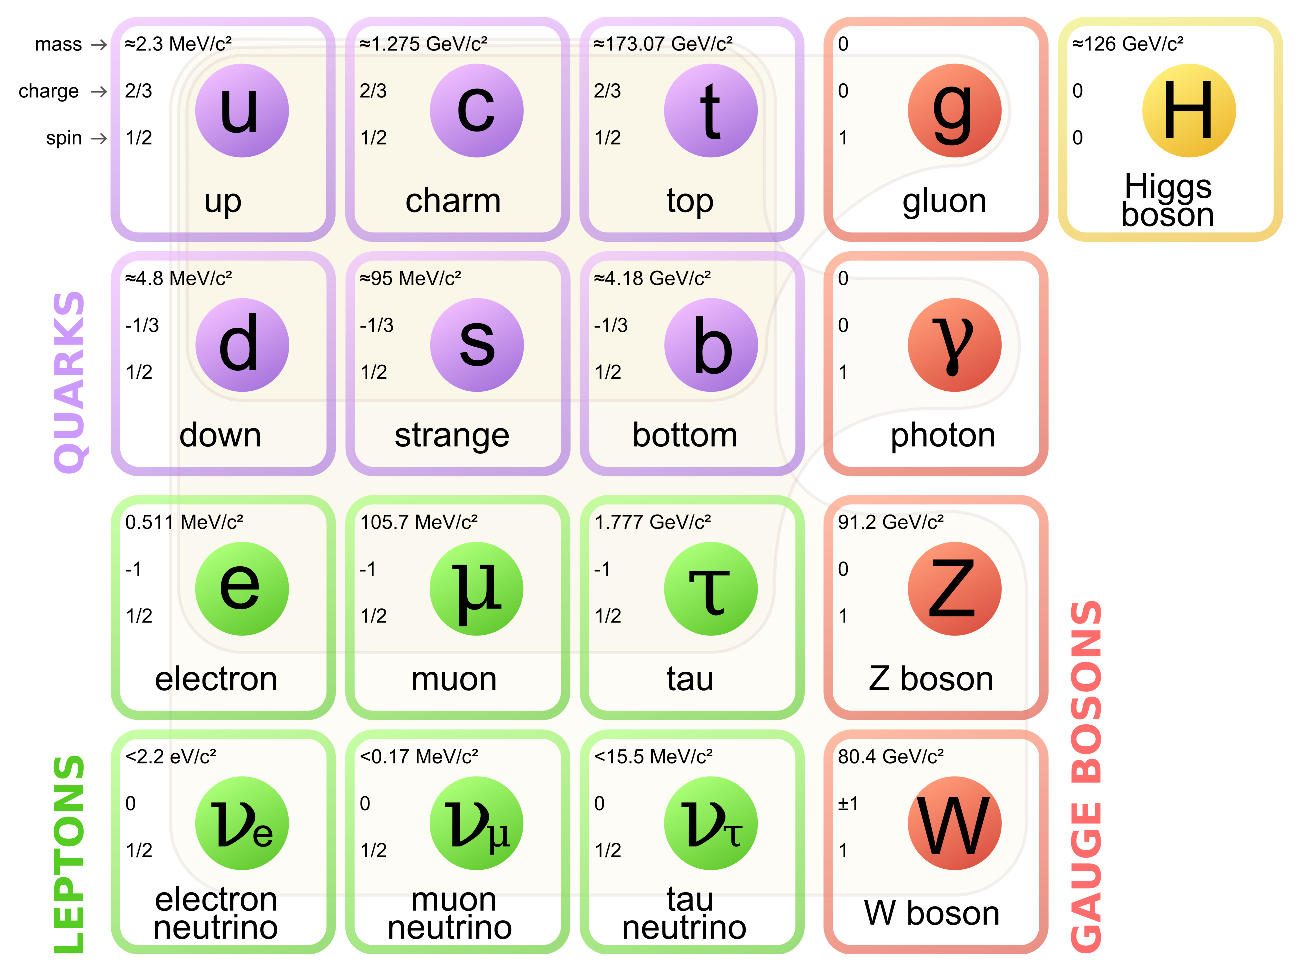
\includegraphics[width=0.8\textwidth]{img/standard_model}
 \caption{Standard Model of Particle Physics~\cite{Wikipedia:StandardModel}.} 
 \label{fig:standard_model}
\end{center}
\end{figure}

Figure~\ref{fig:standard_model} shows an illustration of the Standard Model, which includes
3 generations of leptons (electron, muon, tau), 3 generations of quarks, 4 interaction bosons, ($\gamma$, Z, $\mathrm{W}^{\pm}$, g) and the Higgs boson
recently observed by the ATLAS and CMS Collaborations \cite{ATLAS:2012b,CMS:2012d}.
Each generation of particles (either quarks or leptons) differs from the others for the strength of its coupling to the Higgs boson,
which result in a different observed mass.

At hadron colliders charm quarks are produced as a result of a parton hard scattering. Likewise lighter quarks or gluons, charm quarks
fragment into collimated sprays of hadrons called jets. The charm content of the jet is conserved throughout the fragmentation process,
which is dominated by Quantum Chromo-Dynamics, the theory of strong nuclear interactions.
The charm content of a jet can be identified looking for the presence of charmed hadrons, i.e. hadrons that have
a charm quark among their valence quarks. Since all charmed hadrons have short lifetimes ($\tau \lesssim 10^{-12}$~s) their presence is inferred
using a combination of Particle Identification (PID) techniques and topological and kinematical pattern selections on their decay products.

Charm jets have peculiar properties that result form the heavier mass of the originating parton (a charm quark).
Their production cross-section is significantly smaller than lighter quarks or gluons. The internal
properties of the jets are also affected, in particular the fragmentation is expected to be harder for charm jets compared to inclusive jets.

\begin{figure}[tbh]
\begin{center}
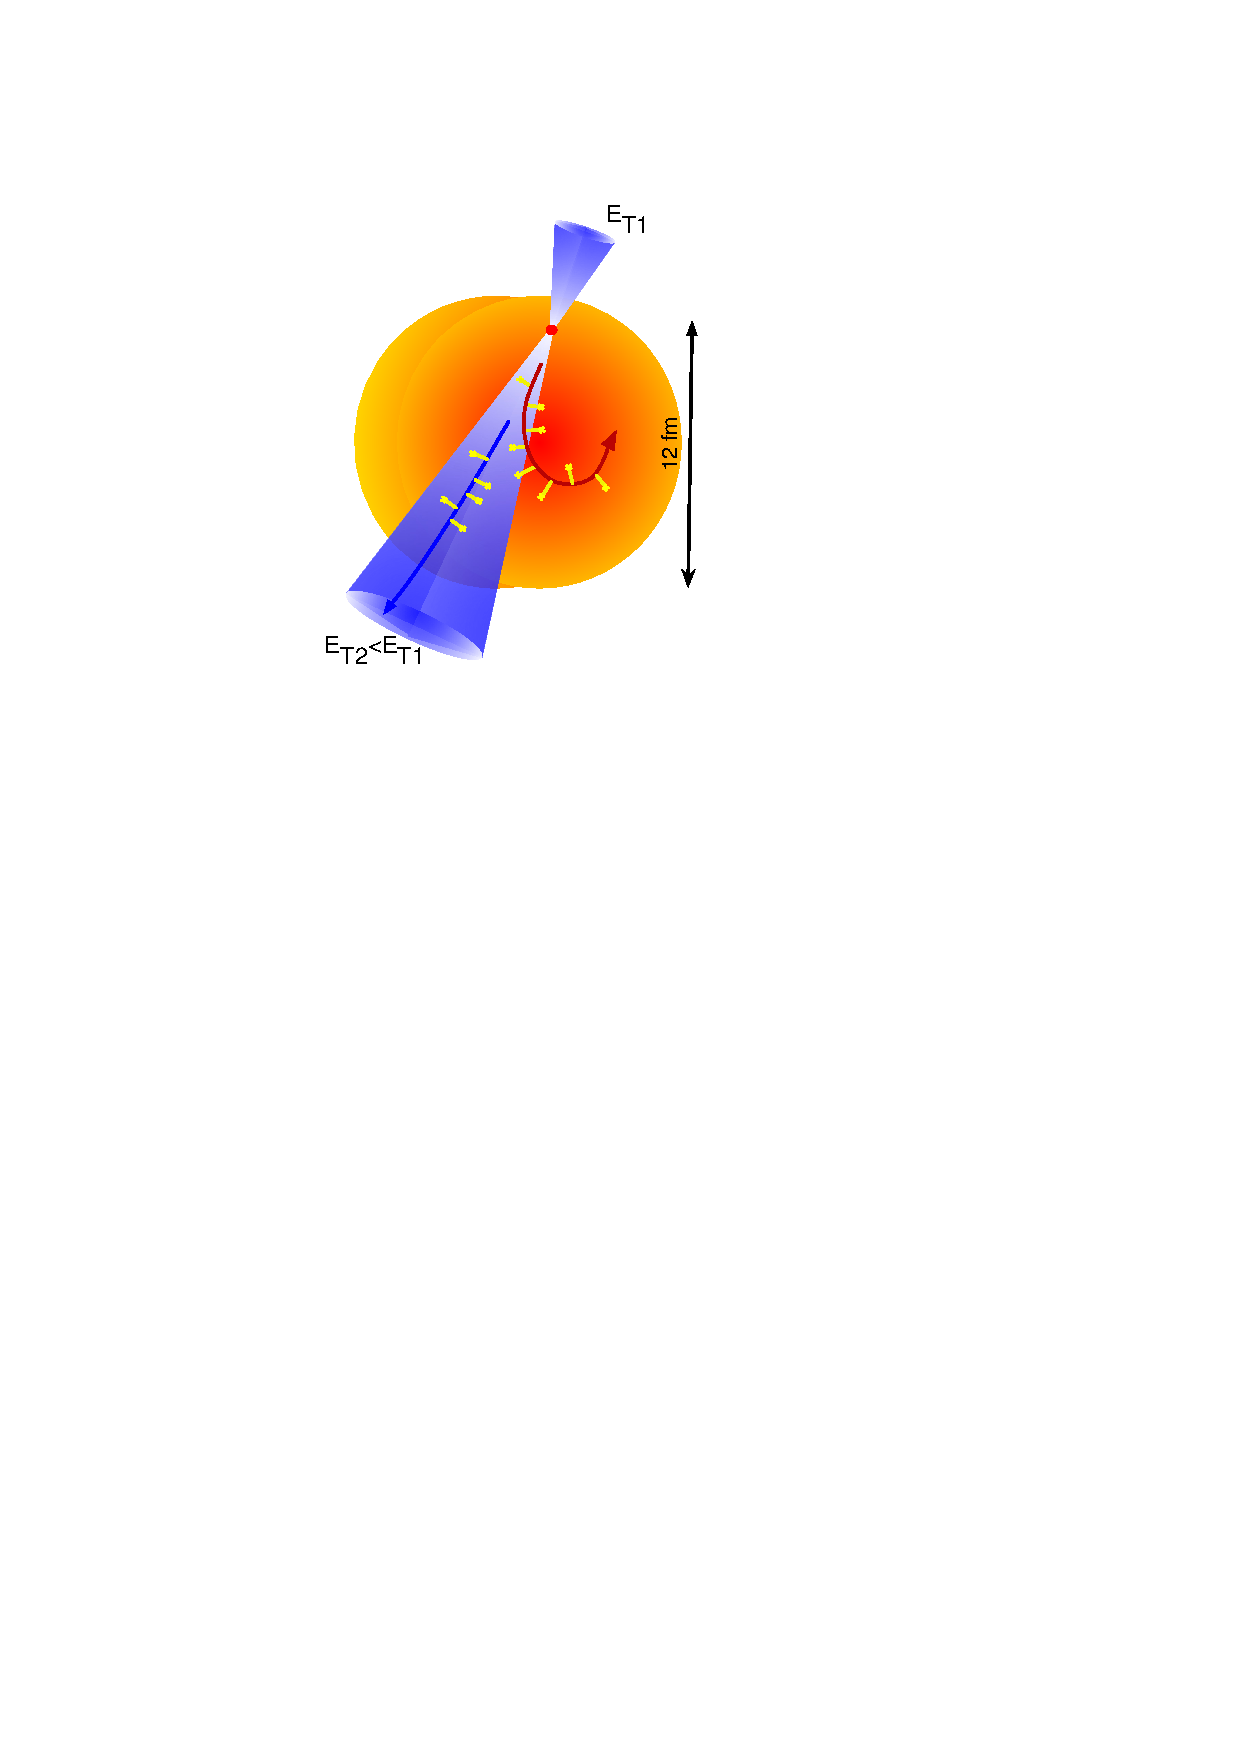
\includegraphics[width=0.5\textwidth]{img/jetquenching}
 \caption{Hard scattered partons interact with the QGP generated in ultra-relativistic heavy-ion collisions.} 
 \label{fig:jetquenching}
\end{center}
\end{figure}

Heavy quarks are also an ideal probe~\cite{} of the hot and dense matter, known as Quark-Gluon Plasma (QGP)~\cite{}, that is created in ultra-relativistic heavy-ion collisions. 
Hard scattered partons, including heavy quarks, are produced early in the collision. They interact with the QGP, which increases their virtuality and interferes with the
parton fragmentation process. This effect, known as \emph{jet quenching}, leads to a broadening and softening of the jet fragmentation~\cite{}, as depicted in Fig.~\ref{fig:jetquenching}. A number of
experimental evidences of jet quenching has been produced in last decade~\cite{}.
High-energy charm jets behave very much like jets originated by light quarks~\cite{}; however at lower energies, comparable to the charm quark mass, the charm quark is expected
to interact less strongly with the QGP, a phenomenon known as dead-cone effect~\cite{}. 
\begin{comment}
The difference between the interaction of a light quark with the QGP and that of
a charm quark is driven by its mass, and is similar to the difference observed in Quantum Electro-Dynamics between muons and electrons interacting with regular matter.
\end{comment}

Charm quarks are produced abundantly at the \emph{Large Hadron Collider}, which provides \pp, \pPb\ and \PbPb\ collisions at unprecedented high collision energies and luminosities.
At the LHC, the PID and low-momentum tracking capabilities are among the strongest points of ALICE~\cite{} compared to the other LHC experiments; 
this advantage is counterbalanced by an overall slower detector which does not allow to probe the full luminosity delivered by the LHC. 
Especially vertexing, tracking and PID are crucial to efficiently identify the decay products of charmed hadrons; tracking and calorimetry are used together to reconstructed the energy flow from which jets can be identified.
ALICE is very well endowed to perform a precise measurement of charm jets in a (mostly) unexplored kinematical region. Furthermore ALICE performances
are optimized for heavy-ion collisions, where charm jet measurements can provide important insights about the QGP.

\section{The Large Hadron Collider}
The \emph{Large Hadron Collider} (LHC) at CERN is the world's largest particle collider ever built.
It is housed in a tunnel with a circumference of 27 km, between 50 and 175 m beneath
the France-Switzerland border near the city of Geneva. The tunnel was built in the 1980s and was used until 
the late 1990s to house the Large Electron-Positron Collider (LEP). The construction of the LHC took about 10 years and started
during the decommissioning phase of LEP. 

Two parallel beam pipes run through the tunnel,
where particles are allowed to travel in opposite directions, intersecting at four points where four different experiments
can detect and measure the collisions (\mbox{ATLAS}, \mbox{ALICE}, \mbox{CMS}, \mbox{LHCb}). More than 1,000 superconducting dipole magnets
are used to keep the particles in their circular trajectories, plus about other 400 superconducting quadrupole and higher multipole
magnets, which are needed to keep the beams focused and provide other optical corrections.

Protons and lead ions undergo several pre-acceleration steps before being injected into the LHC at the energy of 900 GeV (355 GeV per nucleon for lead ions).
They are injected in bunches, spaced by 25 ns (or multiple of it) for a maximum of 2,808 bunches when operating at full luminosity in \pp\ collision mode.
Acceleration is provided through radio frequency cavities. At its highest energy (currently 6.5 TeV for proton beams) the dipole magnets need to generate
a magnetic field of 7.7 T.

At time of writing (July 2016) the LHC is in its Run-2 phase. The first operational phase of the LHC (Run-1) started in November 2009 and was 
concluded in February 2013. In this first phase the LHC successfully provided \pp, \pPb\ and \PbPb\ collisions.
Between 2013 and 2015 the LHC operations were stopped to allow for upgrades to the machine and to the four experiments (Long Shutdown 1, or LS1).
Run-2 started in April 2015 and is scheduled to extend till the end of 2018. Table~\ref{tab:LHCop} shows details of the LHC operations in Run-1 and Run-2.
After Run-2 another 2-year stop is foreseen (LS2) to allow for more upgrades, before the third operational phase (scheduled to start in 2021).

\begin{table}
\centering
\begin{tabular}[tbh]{lrr}
Collision system	&	Years		&	\s\ (TeV)	\\
\hline
\hline
\\
\multicolumn{3}{l}{Run-1} \\
\hline
\multirow{4}{*}{\pp}	&	2009			&	0.9		\\
				&	2010, 2011	&	7		\\
				&	2011			&	2.76		\\
				&	2012			&	8		\\
\hline
\PbPb			&	2010, 2011	&	2.76 		\\
\hline
\pPb				&	2012\tablefootnote{Pilot run}, 2013	&	5.02	\\
\hline
\\
\multicolumn{3}{l}{Run-2} \\
\hline
\multirow{2}{*}{\pp}	&	2015, 2016				&	13	\\
				&	2015						&	5.02	\\
\hline
\PbPb			&	2015						&	5.02	\\
\hline
\pPb				&	2016\tablefootnote{Planned for fall 2016}		&	5.02, 8	\\
\hline
\end{tabular}
\caption{LHC Run-1 and Run-2 operations.
\label{tab:LHCop}}
\end{table}

\section{The ALICE Experiment}
ALICE (\emph{A Large Ion Collider Experiment}) is the experiment dedicated to the study of heavy-ion collisions at the LHC.
Figure~\ref{fig:alice} shows a schematic of the ALICE detector.
ALICE is a complex experiment made of several independent detector sub-systems that are operated synchronously.
The main detectors are in the central barrel and cover the mid-rapidity region ($\lvert \eta\rvert \lesssim 1$).
This is the list of the central-barrel detectors, from the innermost to the outermost:
\begin{itemize}
\item Inner Tracking System (ITS);
\item Time Projection Chamber (TPC);
\item Transition Radiation Detector (TRD);
\item Time Of Flight (TOF);
\item Electromagnetic Calorimeters (EMCal, DCal, PHOS) and High Momentum Particle Identification Detector (HMPID).
\end{itemize}
The central-barrel detectors are placed inside a large conventional solenoid magnet which provides a magnetic field of 0.5 T,
used to bend charged tracks in order to reconstruct their momentum.

Other detectors are placed at forward rapidity and are mainly used for triggering and for event characterization 
(multiplicity, centrality and event plane):
\begin{itemize}
\item Photon Multiplicity Detector (PMD);
\item Forward Multiplicity Detector (FMD);
\item V0 and T0 (multiplicity and triggering);
\item Zero Degree Calorimeter (ZDC).
\end{itemize}
A 5-layer muon tracking station is installed at forward rapidity ($-2.5 < \eta < 4$), inside a dipole magnet.

A full description of ALICE and of its performances during LHC Run-1 is available at Refs.~\cite{}.\

\begin{figure}[tbh]
\begin{center}
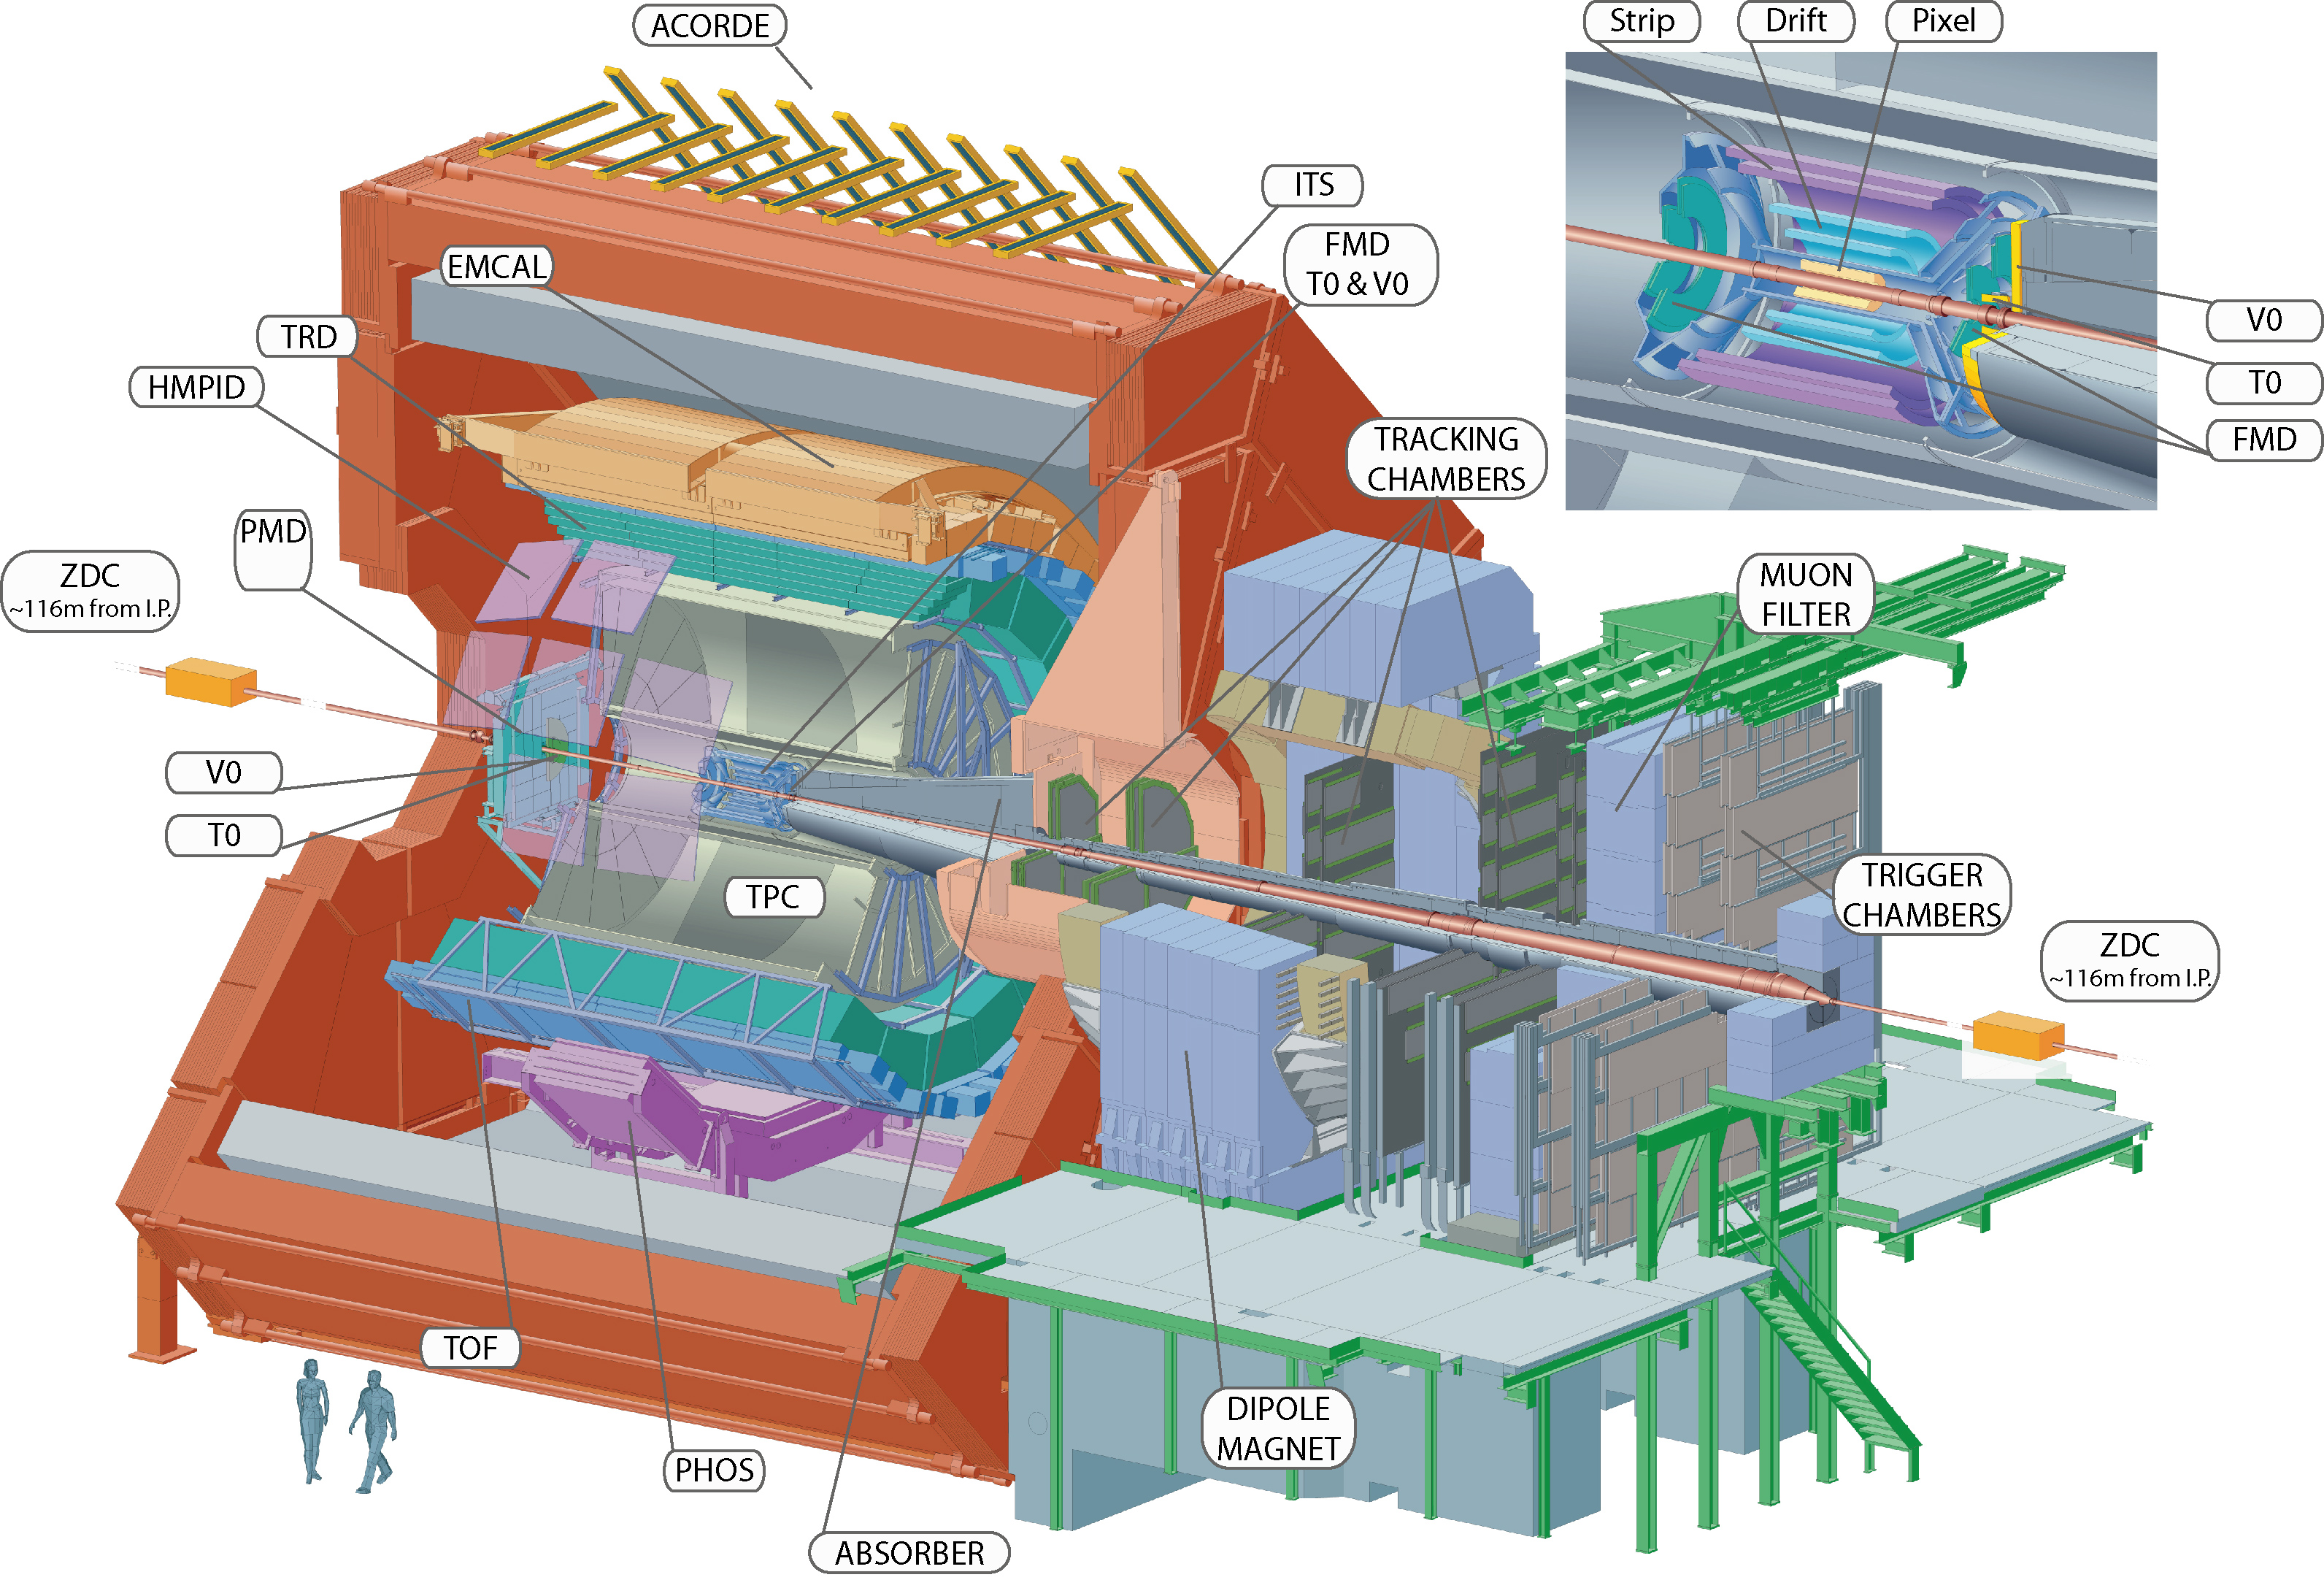
\includegraphics[width=0.7\textwidth]{img/alice}
 \caption{3D ALICE Schematic; central-barrel detectors are visible inside the red solenoid magnet;
 the muon tracking station is on the right side; in the upper-right corner there is a zoomed inlay of the ITS.} 
 \label{fig:alice}
\end{center}
\end{figure}
\begin{comment}
\subsection{Inner Tracking System}
The ALICE \emph{Inner Tracking System} (ITS) is a 6-layer silicon detector: two \emph{Silicon Pixel Detectors} (SPD),
two \emph{Silicon Drift Detectors} (SDD) and two \emph{Silicon Strip Detectors} (SSD).

\subsection{Time Projection Chamber}
The ALICE \emph{Time Projection Chamber} (TPC) is the biggest detector of its kind ever built, with a $90\,\mathrm{m}^{3}$ drift volume.
The chamber is filled with Ne--CO$_{2}$ (Run-1) or Ar--CO$_{2}$ (Run-2) and is divided in two parts by the central cathode, which is kept at -100 kV.
The ionization produced by charged particles transversing the gas is collected at the end plates, which are equipped with multiwire proportional chambers (MWPC).

\subsection{Time Of Flight}
The ALICE \emph{Time Of Flight} (TOF) detector is based on Multigap Resistive Plate Chamber (MRPC) technology and it is used for
particle identification at intermediate momenta (combining the time of flight measurement with the momentum information from the TPC and ITS tracking). 

\subsection{Electromagnetic Calorimeters}
ALICE has three electromagnetic calorimeters that share the azimuthal angle at mid-rapidity. Table~\ref{} summarizes the acceptance
covered by each calorimeter and other physical parameters.

The \emph{Photon Spectrometer} (PHOS) has small acceptance and high resolution
and is especially designed to measure photons.

The \emph{Electromagnetic Calorimeter} (EMCal) and \emph{Di-jet Calorimeter} (DCal) are made of 12,288 and 5,376 towers respectively.
Each tower contains 70 layers that alternate lead plates (to enhance the electromagnetic shower) and scintillator plates. The towers are all identical and have dimensions xx,
which correspond to a thickness of $\sim 20\, X_{0}$ (radiation lengths) and an acceptance of $\Delta\eta \sim 0.014$, $\Delta\phi \sim 0.014$.
The light produced by the electromagnetic shower in the scintillator plates is collected by wavelength-shifting optical-fiber cables that runs through the length of each tower 
in holes carved at the four edges. The four optical fiber cables of each tower are connected optically to an Avalanche Photo-Diode (APD) which converts the optical
signal into an electrical impulse.

The DCal was installed during LS1 and went through a commissioning phase in the first few weeks of data taking in 2015, before becoming fully operational. It covers
an azimuthal region opposite to the EMCal and surrounding PHOS. By combining PHOS and DCal acceptances one effectively covers $\lvert \eta\rvert < 0.7$ and 
$\Delta\phi \sim 67^{\circ}$ in azimuth, thus allowing to perform correlation measurements of back-to-back jets.

\subsubsection{The EMCal-DCal trigger system}
\label{sect:EMCalTriggerSystem}
Both EMCal and DCal can provide triggers for global data taking. ALICE has implemented two trigger levels, L0 and L1, both active for EMCal-DCal.
\end{comment}
\section{D-tagged jets with ALICE}
\subsection{Physics goals}
The measurement of the charm production cross section in \pp\ collisions is an important sensitive test of perturbative QCD (pQCD) calculations.
At the LHC energies, the measurement of charm production at low \pt\ probes the parton distribution functions
of the proton at small values of parton fractional momentum $x$ and squared momentum transfer $Q^2$.
For illustration, using a simplified $2 \rightarrow 2$ kinematics at leading order, c quarks ($m_{\mathrm{c}} \approx 1.5$~\GeVcsq) with
$\pt \sim 2$~\GeVc\ and rapidity $y \sim 0$ probe the parton distribution functions at $x \sim 7 \times 10^{-4}$ and
$Q^2 \sim (5~\mathrm{GeV})^2$.
Perturbative QCD calculations have substantial uncertainties at low \pt, owing to both the large effect of the
choice of the factorization and renormalization scales at low $Q^2$ and to the sizeable uncertainties on the
gluon PDFs at small $x$~\cite{}. 
\begin{comment}
Monte Carlo particle generators, such as PYTHIA~\cite{Sjostrand:2006} or POWHEG~\cite{},
also show only partial agreement with the measurement~\cite{}. 
This poses problems for the High Energy Physics community since these Monte Carlo generators are widely employed as input for detector response simulations.
\end{comment}
Furthermore, the measurement of the charm cross section in \pp\ collisions provides the baseline to look for collective effects in ultra-relativistic
heavy-ion collisions, particularly the ones related to parton energy loss in the QGP. In this context, another crucial aspect is the precise determination of the
total charm-production cross section, needed to model charmonium regeneration in the QGP~\cite{}.
Finally, the measurement of the charm differential cross section down to low \pt, is also relevant for cosmic-ray and neutrino
astrophysics: high-energy neutrinos from the decay of charmed hadrons produced in particle showers in the atmosphere constitute an important
background for neutrinos from astrophysical sources~\cite{}.
\begin{comment}
The inclusive transverse momentum (\pt) and rapidity (\y) differential cross sections can be calculated 
in the collinear factorization approach as a convolution of three terms: i) the parton distribution functions (PDF) of the incoming protons; 
ii) the partonic hard scattering cross section and iii) the fragmentation function, which models the non-perturbative transition of a heavy
quark to a given heavy-flavor hadron species~\cite{}. 

At LHC energies, implementations of these calculations include:
\begin{itemize}
\item the general-mass variable-flavor-number scheme (GM-VFNS) at next-to-leading order (NLO) accuracy~\cite{};
\item the fixed order with next-to-leading-log resummation (FONLL)~\cite{};
\item the \kt-factorization at leading order (LO) approximation, with unintegrated gluon distributions (UGDFs) which account 
for transverse momenta of the initial partons~\cite{}.
\end{itemize}
\end{comment}

Most of the charm-related measurements performed at the LHC so far report the production cross section of hadrons
containing heavy quarks~\cite{}. 
The kinematic properties of the jets are closer to those of the originating c quark, when compared to the measurement of the charmed hadrons alone.
Therefore, by measuring the kinematic properties of jets containing heavy-flavor hadrons 
one reduces the dependence on the details of the fragmentation, which is a highly non-perturbative phenomenon, known only within large uncertainties~\cite{}.
Furthermore, the details of the charm quark fragmentation can be the subject of a more careful study in which the kinematic observables 
of both the jet and the charmed hadron are available at the same time. In particular the measurement of the fraction of the jet momentum carried 
by the charmed hadrons can provide important insights on the charm production mechanism~\cite{}.

\subsection{Analysis technique}
The analysis relies on the well established D meson reconstruction techniques~\cite{}, as well as
jet reconstruction methods~\cite{}, both developed by the ALICE Collaboration. In particular I have
myself contributed significantly to the measurement of jets in \PbPb\ collisions~\cite{} and to the
development and maintenance of the related jet reconstruction software.

Some of the details of the analysis techniques are still under development. In the following section
I will outline the current plan which may change once the analysis proceeds and more information becomes available.

\subsubsection{Data and event selection}
ALICE has collected data in several collision system and at different center of mass energies.
Data taking periods differ from each other also because the conditions of the detector change in time as a result of upgrades,
sub-system sectors that becomes inactive or get fixed. The trigger conditions can change as well, depending on the
physics goals set by the Collaboration and on the instantaneous luminosity expected to be delivered by the LHC.
All these factors need to be taken into account to chose a good dataset that best suits a new physics analysis.

I have started to develop the analysis techniques using the data collected by ALICE in 2010 when the LHC was
delivering \pp\ collisions at 7 TeV in the center of mass. At that time only 2 EMCal super-modules out of 12 were installed.
This means that the EMCal cannot be used to reconstruct the jet momentum carried by neutral constituents; therefore jets are
reconstructed only using charged particles measured by the central tracking system (TPC and ITS).
Jets reconstructed using only charged particles are usually referred to as \emph{charged jets}. This dataset is very
well understood within ALICE, in terms of detector performances, and therefore it looked like a perfect working bench
to test the core analysis techniques without the additional complications coming from using the calorimeter data.

To reconstruct full jets, i.e. jets reconstructed out of charged particles from the tracking system and neutral particles from their
electromagnetic showers in the EMCal-DCal, one has to look at more recent datasets taken with an extended calorimeter acceptance.
The data taken in 2012 with \pp\ collisions at 8 TeV is a very good candidate. Even more interesting could be the data currently (2016)
being collected with \pp\ collisions at 13 TeV. The EMCal-DCal is also providing a trigger dedicated to jet physics, 
to which I contributed in the commissioning phase earlier this year (see Section~\ref{sect:TriggerCommisioning}).

For the data collected in 2010, only \emph{minimum bias} (MB) triggers were active. These triggers
try to keep the bias coming from online event selection to a minimum, i.e. every time detectors
are exposed to some activity correlated with an LHC bunch crossing, the event is read-out and stored.
The detector sub-systems that are involved in this type of trigger are the SPD, the V0 and the T0.
The data collected in 2012 and the data currently being collected also include triggers
provided by the EMCal-DCal (see Section~\ref{sect:EMCalTriggerSystem} for details).
In this case events are read-out only if a large enough shower has been detected by the calorimeters.
Trigger biases need to be understood and corrected for, using a combination of data-driven methods and simulations.
For the data collected in 2012 and 2016 I plan to use events triggered by EMCal L1 jet algorithm.

\subsubsection{Track selection}
For more details about the tracking algorithm used by ALICE see Ref.~\cite{}.

Track quality cuts are applied to ensure good momentum resolution. These cuts
depend on the requirements set by a specific physics analysis.
Two types of tracks are used for this analysis. \emph{Global} tracks have the best
momentum and spatial resolution. They include at least one space point in the SPD (first two
layers of the ITS, closer to the beam pipe) and at least a total of three in the whole ITS. They are required also to
match with a track in the TPC, which has to include at least 70 space points and no less than 80\% of the geometrically findable 
space points in the TPC. Decay products of the D mesons are found among this category of tracks.

Due to the non-uniform SPD response, the reconstruction efficiency of the above defined \emph{global} tracks shows a strong azimuthal dependence,
as shown in Fig.~\ref{}. This non-uniform acceptance can interfere with the jet finding algorithm. To avoid such effects a second type of tracks is added for jet finding.
For this type of tracks the requirement on the SPD is lifted, while keeping all the other requirements unchanged. To improve momentum resolution,
these tracks are constrained to the primary vertex, which is reconstructed using \emph{global} tracks. These tracks are called \emph{hybrid} because
they are a combination of \emph{global} tracks and \emph{constrained} tracks.

\subsubsection{D meson candidate identification}
ALICE has successfully measured a number of charmed mesons~\cite{}.
The \Dzero\ meson has the best signal/background ratio down to low momentum and
is also the most abundant.
It is identified through its hadronic decay: \Dzero $\rightarrow$ \pip \kam. The branching ratio of this decay
is relatively small, BR(\Dzero $\rightarrow$ \pip \kam) = xx~\cite{}. Both the \Dzero\ and its
anti-particle $\overline{\Dzero}$~are considered.

The first step of the analysis is to select events that contain at least one \Dzero\ meson candidate.
\Dzero\ meson candidates are identified looking for opposite-sign track pairs (\emph{daughters}) among all reconstructed \emph{global} tracks.
In order to suppress the background from combinatorial matches, topological and PID cuts are applied.
The topological cuts select pairs that form a \emph{secondary vertex} displaced from the reconstructed
primary vertex. Depending on the momentum of the D meson candidate, different cuts are applied on the
\emph{distance of closest approach} (DCA) between each of the daughters and the primary vertex. These cuts
varies from DCA $>$ xx for xx to xx for xx.
When the PID information is available it is used to reject pairs that do not satisfy the requirement of being a pion-kaon pair.

The pairs that pass the selections are then used in the next steps.
The four-momentum of the \Dzero\ candidate is calculated summing the four-momenta of the two daughters.
When available, PID is used to assign mass values to the \Dzero\ candidate daughters. When PID is not conclusive,
the pair is used twice with either mass combinations (\pip \kam or \pim \kap). Using the four-momentum of the \Dzero\ candidate
the \emph{invariant mass} is calculated according to the usual special relativity formula: $m^2 = E^2 - \bm{p}^2$.

\subsubsection{Jet reconstruction}
For each \Dzero\ candidate a set of particle four-momenta is prepared and fed as input for the jet finding algorithm.
This set includes the four-momentum of the \Dzero\ candidate and all reconstructed \emph{hybrid} tracks,
excluding the two daughters of the \Dzero. The jet finding algorithm returns a set of jet candidates, with the particle constituents
assigned to each jet. The jet containing the \Dzero\ candidate can thus be identified and associated with the \Dzero\ candidate for the next steps.

\begin{comment}
Several jet finding algorithms have been developed and used in high energy physics in the last few decades.
\emph{Cone jet algorithms} were the first to be developed. Although many different versions exists, the basic idea behind them
is to place a cone in the $\eta\phi$ space where particles are reconstructed. The procedure is usually iterative and makes use of \emph{seeds}
among the particles with the highest momentum, although seed-less versions exist too~\cite{}.
With few exceptions, cone algorithms suffer from experimental and theoretical issues and have been
replaced by \emph{sequential recombination algorithms}. For these algorithms a \emph{measure} is defined among all reconstructed particles.
\end{comment}

Initially I will focus on using only tracks of charged particles for jet reconstruction. Since they miss the momentum
fraction carried by neutral particles, the kinematics of charged jets is less tightly correlated with the kinematics
of the original parton and depends more strongly on the jet fragmentation; however charged jets have also a a number advantages
and have been the subject of recent theoretical developments~\cite{}.
In a second phase I plan to extend the analysis by including the calorimeter data in jet finding (as done in Refs.~\cite{}).

\subsubsection{Invariant mass analysis}
\Dzero\ candidates and their associated jets are then sorted according to their kinematic variables in different bins:
\begin{enumerate}
\item for a single-differential D-tagged jet \pt\ spectrum, the candidates will be divided in bins according to their associated jet \pt;
\item for a double-differential spectrum in jet \pt\ and \zpar$=\frac{\bm{p}_{\rm jet}\cdot{\bm{p}}_{\rm D^0}}{\bm{p}_{\rm jet}^2}$ candidates will
be sorted in bins defined in these two variables.
\end{enumerate}
For each bin defined above, a separate invariant mass analysis is performed. An example is shown in Fig.~\ref{} for the single-differential
jet \pt\ spectrum case. 

\subsubsection{Final corrections and systematic uncertainties}

\subsection{Timeline}
bla bla
\section{Service work}
\subsection{The EMCal-DCal 2016 trigger commissioning}
\label{sect:TriggerCommisioning}
\subsection{TPC upgrade for LHC Run-3}

\bibliography{biblio}{}
\bibliographystyle{utphys}

\end{document}
